\documentclass[letterpaper,11pt]{article}
\oddsidemargin -1.0cm \textwidth 17.5cm

\usepackage[utf8]{inputenc}
\usepackage[activeacute,spanish, es-lcroman]{babel}
\decimalpoint
\usepackage{amsfonts,setspace}
\usepackage{amsmath}
\usepackage{amssymb, amsmath, amsthm}
\usepackage{comment}
\usepackage{float}
\usepackage{amssymb}
\usepackage{dsfont}
\usepackage{anysize}
\usepackage{multicol}
\usepackage{enumerate}
\usepackage{graphicx}
\usepackage[left=1.5cm,top=2cm,right=1.5cm, bottom=1.7cm]{geometry}
\setlength\headheight{1.5em} 
\usepackage{fancyhdr}
\usepackage{multicol}
\usepackage{hyperref}
\usepackage{wrapfig}
\usepackage{subcaption}
\usepackage{siunitx}
\usepackage{cancel}
\usepackage{mdwlist}
\pagestyle{fancy}
\fancyhf{}
\renewcommand{\labelenumi}{\normalsize\bfseries P\arabic{enumi}.}
\renewcommand{\labelenumii}{\normalsize\bfseries (\alph{enumii})}
\renewcommand{\labelenumiii}{\normalsize\bfseries \roman{enumiii})}


\begin{document}

\fancyhead[L]{\itshape{Facultad de Ciencias F\'isicas y Matem\'aticas}}
\fancyhead[R]{\itshape{Universidad de Chile}}

\begin{minipage}{11.5cm}
    \begin{flushleft}
        \hspace*{-0.6cm}\textbf{FI1000-6 Introducción a la Física Clásica}\\
        \hspace*{-0.6cm}\textbf{Profesora:} Paulina Lira\\
        \hspace*{-0.6cm}\textbf{Auxiliares:} Juan Cristóbal Castro \& Alejandro Silva\\
        \hspace*{-0.6cm}\textbf{Ayudantes:} Francisca Bórquez, Catalina Molina \& Erick Pérez\\
        
    \end{flushleft}
\end{minipage}

\begin{picture}(2,3)
    \put(366, 10){
\includegraphics[scale=0.9]{2020-1/Imágenes/logo/dfi-fcfm.pdf}}
\end{picture}

\begin{center}
	\LARGE\textbf{Auxiliar \#4}\\
	\Large{MCUA y Movimiento Relativo}
\end{center}

\vspace{-1cm}
\begin{enumerate}\setlength{\itemsep}{0.4cm}

\rfoot[]{pág. \thepage}

\item[]

\item Un ventilador de techo posee unas aspas de largo $L$. Un apagón provoca que las aspas se detengan en un tiempo $\tau$, tras haber estado rotando a una frecuencia $f$.

\begin{enumerate}
    \item Obtenga la aceleración angular y el número de rotaciones completadas desde que ocurre el apagón.
    
    \item Para un tiempo $t = \tau/2$, obtenga: rapidez tangencial, aceleración radial, aceleración tangencial y aceleración total.
\end{enumerate}

\item Un tren se mueve sobre una línea recta horizontal con velocidad constante $v_0\hat{i}$. En un instante el maquinista lanza una maleta con velocidad $u_0\hat{j}$ verticalmente hacia arriba.

    \begin{enumerate}
        \item De acuerdo al maquinista, ¿cuál es la trayectoria de la maleta?
        
        \item Para un observador en reposo a un costado del tren, ¿cuál es el desplazamiento de la maleta desde que es lanzada hasta que cae de nuevo sobre el tren?
    \suspend{enumerate}
    
    Si ahora la maleta es lanzada por el maquinista con una velocidad $u = -v_0\hat{i} + n v_0\hat{j}$ y cada vagón del tren tiene una longitud $L$:
    
    \resume{enumerate}
        \item Bosqueje en el plano $x-y$ la trayectoria de la maleta registrada por un observador en reposo a un costado del tren.
        
        \item Determine el valor mínimo de $v_0$ para que la maleta caiga sobre el vagón k-ésimo.
        
    \end{enumerate}
    
\item (\textbf{P1-C2 2017-1}) Imagine un mundo que transcurre sobre una plataforma circular de radio muy grande, que gira con velocidad angular $\Omega$ constante. En el entorno de la plataforma existe una aceleración de gravedad $\vec{g}$ constante. Una persona ubicada a una distancia $L$ del centro $O$, en reposo con respecto a la plataforma, lanza una moneda al aire en dirección vertical y con rapidez $v_0$ (respecto a la persona). Determine el tiempo que demora en caer la moneda al suelo y el lugar sobre la plataforma, con respecto a la persona, donde lo hace.

\textbf{\textit{Hint:}} Analice el lanzamiento de la moneda desde un observador ubicado en un sistema $S$ fijo con origen en $O$

\begin{figure}[H]
    \centering
    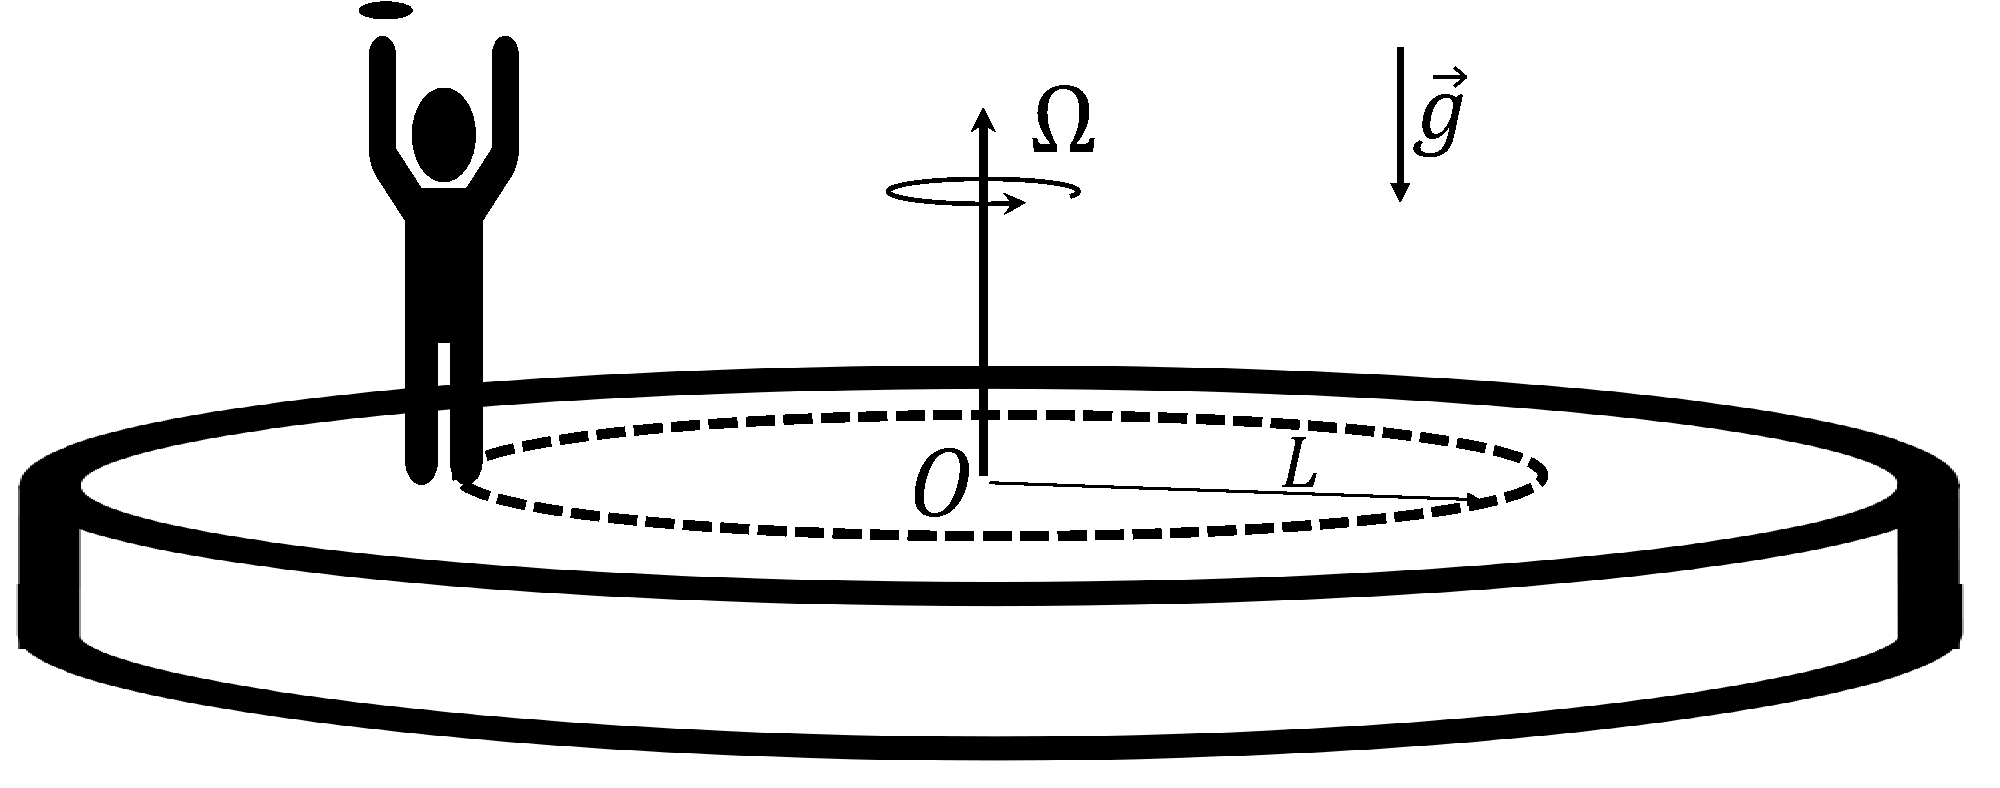
\includegraphics[width = 0.4\linewidth]{2021-1/Imagenes/aux4/moneda-circulo.pdf}
\end{figure}

\end{enumerate}
\end{document}